%!TEX root =../quadrotorbook.tex
\chapter{Scene Reconstruction}
\label{chap:scene_reconstruction}

In this chapter we will consider the problem of reconstruction a local voxel grid representation of the world based on a video sequence collected by the camera.  A high-level architecture for scene reconstruction is shown in Figure~\ref{fig:scene_reconstruction_architecture}.
%
\begin{marginfigure}[0in]
	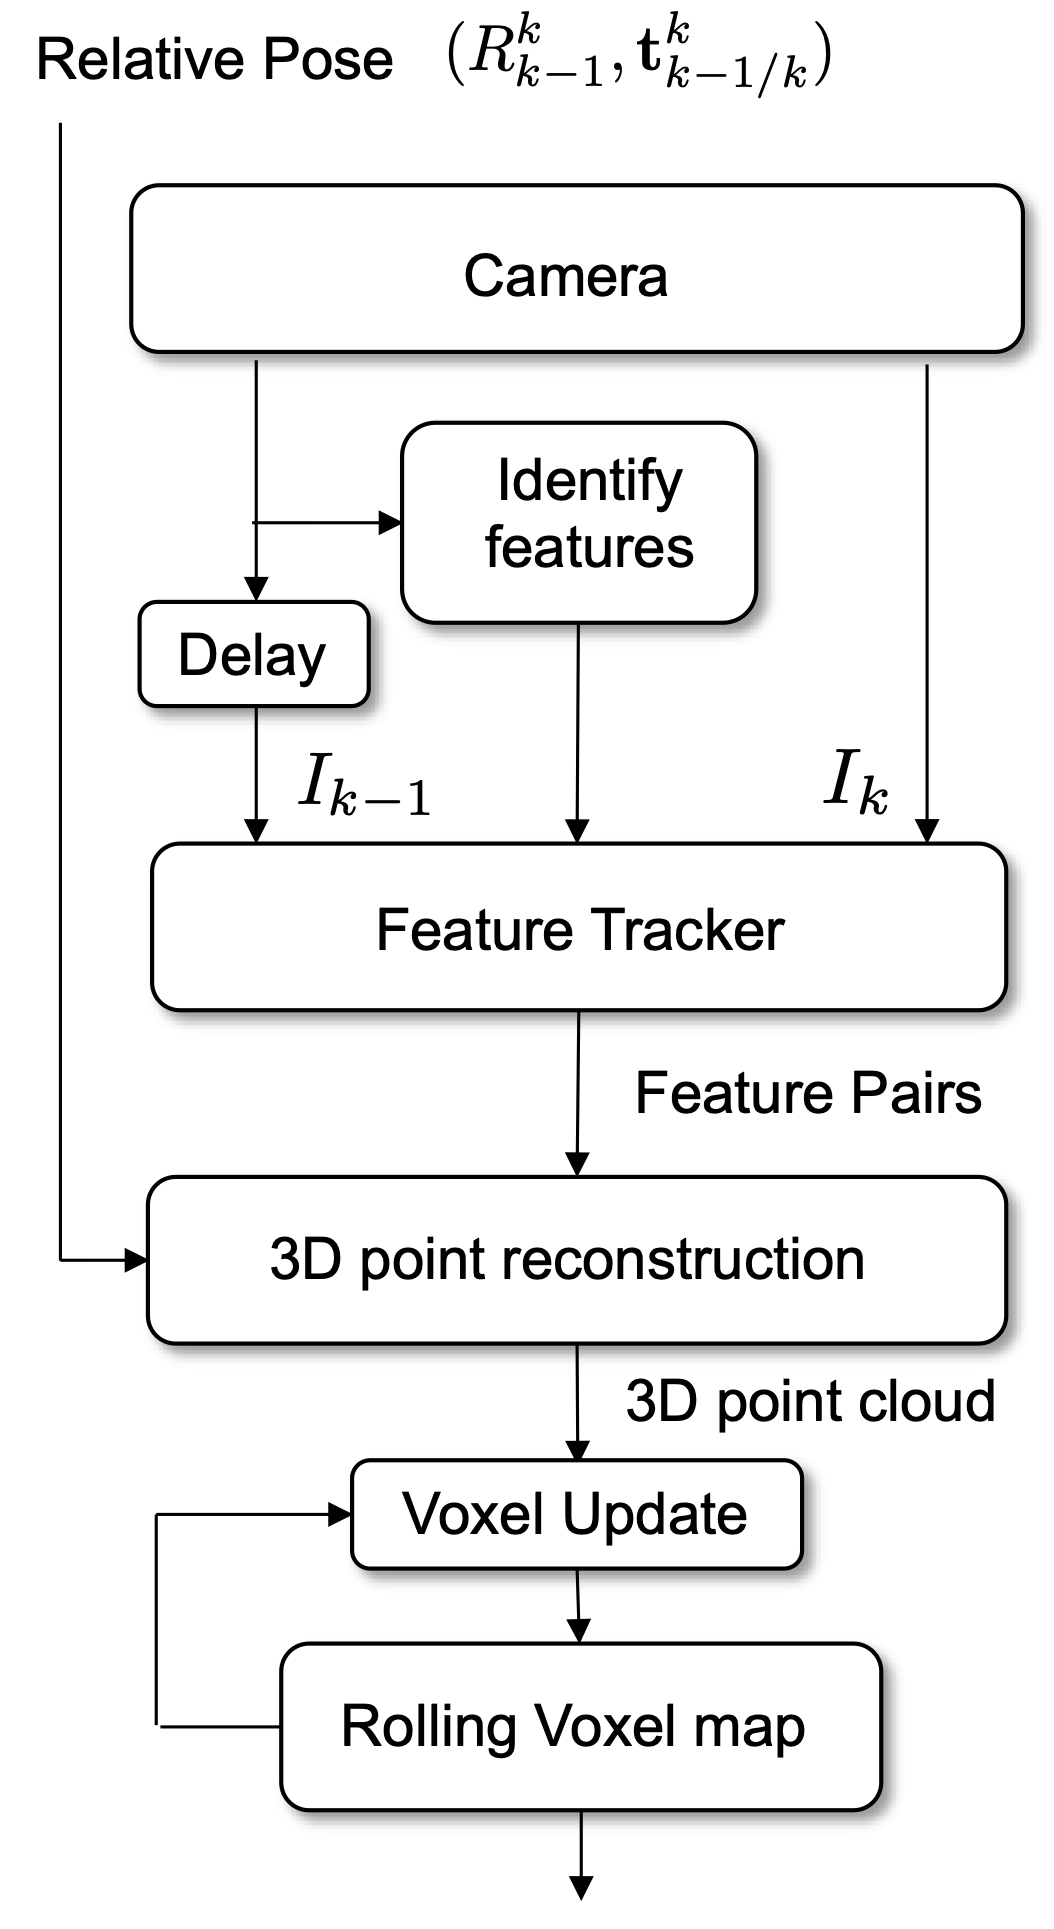
\includegraphics[width=\linewidth]{chap8_scene_reconstruction/figures/scene_reconstruction_architecture}
	\caption{Architecture for Scene Reconstruction}
	\label{fig:scene_reconstruction_architecture}  
\end{marginfigure}
%
The camera image at time $k-1$ is used to identify good features in the image.  Those features are then tracked to the image $I_k$ to produce a set of feature pairs in calibrated normalized homogeneous coordinates, denoted $\mathcal{P}_k = \{(\bar{\epsilonbf}_i^{k-1},\bar{\epsilonbf}_i^{k}), i=1,\dots, N\}$.  The feature pairs are then used to reconstruct the 3D points corresponding to the feature points.  In this chapter we will assume that the camera's rotation and translation between images is known, and therefore the 3D reconstruction algorithm as access to these quantities denoted in Figure~\ref{fig:scene_reconstruction_architecture} as $(R_{k-1}^k \pbf_{k-1/k}^k)$.  The 3D scene points are used to update the rolling voxel grid described in Chapter~\ref{chap:trajectory_planning}.
	
In Section~\ref{sec:imu_integration} we review how IMU integration can be used to obtain the relative pose $(R_{k-1}^k, \pbf_{k-1/k}^k)$.  
%	
Section~\ref{sec:essential_matrix} derives  the essential matrix and discusses some of its properties. 
%
Section~\ref{sec:homography_matrix} describes the homography matrix and some of its properties.  
%
Section~\ref{sec:point_reconstruction} gives several simple point reconstruction algorithms.
%
Section~\ref{sec:voxel_map_updates} describes how to update the rolling voxel map given point cloud information.

Embedded papers describe more sophisticated reconstruction techniques.



%------------------------------------------------
\section{IMU Integration}
\label{sec:imu_integration}
The methods used in this chapter will depend on knowledge of the relative pose between camera frames.  Let $\mathcal{F}_{k}$ be the camera frame at time $k$, then the relative pose is given by $(R_{k-1}^k, \pbf_{k-1/k}^k)$, where $R_{k-1}^k\in SO(3)$ is the rotation matrix from $\mathcal{F}_{k-1}$ to $\mathcal{F}_k$, and $\pbf_{k-1/k}^k\in\mathbb{E}^3$ is the position of $\mathcal{F}_{k-1}$ relative to $\mathcal{F}_k$, expressed in $\mathcal{F}_k$. 

In this section we show how the relative pose $(R_{k-1}^k, \pbf_{k-1/k}^k)$ can be obtained from an IMU rigidly attached to the camera.  The discussion in this section follows in some respects, the development in (Forster 2017)\cite{ForsterCarloneDellaert17}.  
We will assume in this section that the IMU is rigidly attached to the camera and that the IMU has been calibrated and the biases have been removed.  Then the output of the IMU is the 
angular velocity $\omegabf_{c/i}^c$ and the specific acceleration $\abf_{c/i}^c$, 
where $\mathbf{F}_c$ is the camera frame and $\mathcal{F}_i$ is the inertial frame. 
We will assume that the camera moves according to 
\begin{align}
\dot{\pbf}_{c/i}^i &= \vbf_{c/i}^i  \label{eq:camera_motion_p} \\
\dot{\vbf}_{c/i}^i &= g \ebf_3 + R_c^i\abf_{c/i}^c, \label{eq:camera_motion_v} \\
\dot{R}_c^i &= R_c^i \ss{\omegabf_{c/i}^c}. \label{eq:camera_motion_R}
\end{align}
We begin by developing a sampled-data version of the equations of motion.
\begin{lemma}
	Suppose that the camera evolves according to \eqref{eq:camera_motion_p}--\eqref{eq:cam_motion_R} and suppose that over one sample period $(t_\ell, t_{\ell+1})$ of length $T_s=t_{\ell+1}-t_\ell$, that the angular velocity $\omegabf_{\ell/i}^{\ell}\defeq\omegabf_{c/i}^c(t_\ell)$ and the specific acceleration $\abf_{\ell/i}^{\ell}\defeq \abf_{c/i}^c(t_\ell)$ are constant.  Then the discrete evolution equations are given by
	\begin{align}
	R_{\ell+1}^i &= R_{\ell}^i \exp\left(\ss{\omegabf_{\ell/i}^{\ell}} T_s \right)
	\label{eq:R_imu_int_1} \\
	\vbf_{\ell+1/i}^{i} &= \vbf_{\ell/i}^{i} + T_s g \ebf_3 + T_s R_{\ell}^i \abf_{\ell/i}^{\ell} \label{eq:v_imu_int_1} \\
	\pbf_{\ell+1/i}^{i} &= \pbf_{\ell/i}^{i} + T_s\vbf_{\ell/i}^i + \frac{T_s^2}{2} g\ebf_3 + \frac{T_s^2}{2} R_{\ell}^i \abf_{\ell/i}^{\ell} \label{eq:p_imu_int_1}.
	\end{align}
\end{lemma}
\begin{proof}
	We have shown in Lemma~\ref{} that for a constant angular velocity, the solution of Equation~\eqref{eq:camera_motion_R} is \eqref{eq:R_imu_int_1}.
	For a constant input, integrating~\eqref{eq:camera_motion_v} gives
	\begin{align*}
	\vbf_{c/i}^i(t) &= \vbf_{c/i}^i(t_0) + \int_{t_0}^t \left(g\ebf_3 + R_c^i \abf_{c/i}^c\right)d\tau \\
		&= \vbf_{c/i}^i(t_0) + \int_{t_0}^t d\tau \left(g\ebf_3 + R_c^i \abf_{c/i}^c\right) \\
		&= \vbf_{c/i}^i(t_0) + (t-t_0) \left(g\ebf_3 + R_c^i \abf_{c/i}^c\right).
	\end{align*}
	Letting the camera frame at time $t_\ell$ be denoted as $\mathcal{F}_\ell$, and letting $t=t_{\ell+1}$ and $t_0=t_{\ell}$ gives Equation~\eqref{eq:v_imu_int_1}.  Similarly, integrating Equation~\eqref{eq:camera_motion_p} gives
	\begin{align*}
	\pbf_{c/i}^c(t) &= \pbf_{c/i}^c(t_0) + \int_{t_0}^t \vbf_{c/i}^i(\tau)d\tau \\
		&= \pbf_{c/i}^c(t_0) + \int_{t_0}^t \left(\vbf_{c/i}^i(t_0) + \int_{t_0}^\tau \left(g\ebf_3 + R_c^i \abf_{c/i}^c\right)d\sigma \right) d\tau \\
		&= \pbf_{c/i}^c(t_0) + (t-t_0)\vbf_{c/i}^i(t_0) + \frac{(t-t_0)^2}{2}\left(g\ebf_3 + R_c^i \abf_{c/i}^c\right),
	\end{align*}
	and Equation~\eqref{eq:p_imu_int_1} follows by letting $t=t_{\ell+1}$ and $t_0=t_{\ell}$.
\end{proof}
Since the relative pose does not include the inertial frame, we would like to remove references to the inertial frame in Equations~\eqref{eq:p_imu_int_1}--\eqref{eq:R_imu_int_1}.  The next lemma does so.
\begin{lemma}
	Suppose that the camera evolves according to \eqref{eq:camera_motion_p}--\eqref{eq:camera_motion_R} and suppose that over one sample period $(t_\ell, t_{\ell+1})$ of length $T_s=t_{\ell+1}-t_\ell$, that the angular velocity $\omegabf_{\ell/i}^{\ell}\defeq\omegabf_{c/i}^c(t_\ell)$ and the specific acceleration $\abf_{\ell/i}^{\ell}\defeq \abf_{c/i}^c(t_\ell)$ are constant.  Then the discrete evolution from IMU sample $\ell$ to IMU sample $\ell+1$ is given by
	\begin{align}
	R_{\ell}^{\ell+1} &= \exp\left(-\ss{\omegabf_{\ell/i}^{\ell}} T_s \right)
		\label{eq:R_imu_int_2} \\
	\vbf_{\ell/\ell+1}^{\ell+1} &= R_{\ell}^{\ell+1}\left( \vbf_{\ell-1/\ell}^{\ell} 
		+ T_s \left(R_{\ell-1}^\ell \abf_{\ell-1/i}^{\ell-1} - \abf_{\ell/i}^\ell \right) \right)  \label{eq:v_imu_int_2} \\
	\pbf_{\ell/\ell+1}^{\ell+1} &= R_{\ell}^{\ell+1}\left(\pbf_{\ell-1/\ell}^{\ell} 
		+T_s\vbf_{\ell-1/\ell}^{\ell} + \frac{T_s^2}{2}\left(R_{\ell-1}^\ell \abf_{\ell-1/i}^{\ell-1} - \abf_{\ell/i}^{\ell}\right)\right).
		\label{eq:p_imu_int_2}
\end{align}
\end{lemma}
\begin{proof}
	The relative pose between IMU measurements is given by
	\[
	R_{\ell}^{\ell+1} = R_{\ell+1}^{i\top}R_{\ell}^i 
		= \exp\left(-\ss{\omegabf_{\ell/i}^{\ell}} T_s \right)
	\]
	where the second equation follow from Equation~\eqref{eq:R_imu_int_1}.
	For the relative velocity, we have from Equation~\eqref{eq:v_imu_int_1} that
	\begin{align*}
	\vbf_{\ell/\ell+1}^{\ell+1} 
	&= R_{\ell+1}^{i\top}\left(\vbf_{\ell/i}^i - \vbf_{\ell+1/i}^i\right) \\
	&= 	R_{\ell+1}^{i\top}\Big(\vbf_{\ell-1/i}^i + T_s g\ebf_3 + T_s R_{\ell-1}^i 
		\abf_{\ell-1/i}^{\ell-1} 
		\\ &\qquad\qquad
		- \vbf_{\ell/i}^i - T_s g\ebf_3 - T_s R_{\ell}^i \abf_{\ell/i}^{\ell} \Big)  \\
	&= 	R_{\ell}^{\ell+1} \Big(\vbf_{\ell-1/\ell}^{\ell}
		+ T_s \left( R_{\ell-1}^{\ell} \abf_{\ell-1/i}^{\ell-1}
		- \abf_{\ell/i}^{\ell} \right) \Big).
	\end{align*}
	Similarly, the relative translation vector is given by
	\begin{align*}
	\pbf_{\ell/\ell+1}^{\ell+1} 
	&= R_{\ell+1}^{i\top}\left(\pbf_{\ell/i}^i - \pbf_{\ell+1/i}^i\right) \\
	&= R_{\ell+1}^{i\top}\Big(\pbf_{\ell-1/i}^{i} + T_s\vbf_{\ell-1/i}^i + \frac{T_s^2}{2} g\ebf_3 + \frac{T_s^2}{2} R_{\ell-1}^i \abf_{\ell-1/i}^{\ell-1}
	\\ &\qquad\qquad
	-\pbf_{\ell/i}^{i} - T_s\vbf_{\ell/i}^i - \frac{T_s^2}{2} g\ebf_3 - \frac{T_s^2}{2} R_{\ell}^i \abf_{\ell/i}^{\ell} \Big) \\
	&= R_{\ell}^{\ell+1}\Big(\pbf_{\ell-1/\ell}^{\ell} 
	+ T_s \vbf_{\ell-1/\ell}^{\ell} 
	+\frac{T_s^2}{2}\left(R_{\ell-1}^{\ell}\abf_{\ell-1/i}^{\ell-1} - \abf_{\ell/i}^{\ell}\right)\Big).
	\end{align*}
\end{proof}

If there are $m$ IMU samples between camera frame $k-1$ and camera frame $k$, then the relative pose can be estimated using the following algorithm.
\begin{description}
	\item[Initialization.] At frame $k-1$, upon receiving IMU measurement $\ell=0$ at time $t_{k-1}$ initialize the relative pose as
	\begin{align*}
	R_{k-1}^1 &= \exp\left(-\ss{\omegabf_{0/i}^0}T_s\right) \\
	\vbf_{k-1/1}^1 &= 0 \\
	\pbf_{k-1/1}^1 &= 0.
	\end{align*}
	\item[Iteration.] For the $\ell^{th}$ IMU measurement $(\omegabf_{\ell/i}^\ell, \abf_{\ell/i}^\ell)$, $\ell=1,\dots,m$ let 
	\begin{align*}
	R_{k-1}^{\ell+1} &= R_\ell^{\ell+1} R_{k-1}^{\ell} \\
	\vbf_{k-1/\ell+1}^{\ell+1} &=  R_{\ell}^{\ell+1}\vbf_{k-1/\ell}^{\ell} + \vbf_{\ell/\ell+1}^{\ell+1} \\
	\pbf_{k-1/\ell+1}^{\ell+1} &= R_{\ell}^{\ell+1}\pbf_{k-1/\ell}^{\ell} + \pbf_{\ell/\ell+1}^{\ell+1},
	\end{align*} 
	where $R_{\ell}^{\ell+1}$, $\vbf_{\ell/\ell+1}^{\ell+1}$, and $\pbf_{\ell/\ell+1}^{\ell+1}$ are given by Equations~\eqref{eq:R_imu_int_2}--\eqref{eq:p_imu_int_2}.
\end{description}
When $\ell=m$, then $t_m=t_k$ and the algorithm has determined the relative pose $(R_{k-1}^k, \pbf_{k-1/k}^k)$.

\rwbcomment{Note that this is different than other IMU integration methods in that the method uses the difference of accelerometer measurements.  It will be interesting to see if this work!}

\rwbcomment{Add a description of a VIO approach.  The above is just inertial odometry (IO), to correct for biases, need to add the visual correction.}

%------------------------------------------------
\section{Essential Matrix}
\label{sec:essential_matrix}
%Author: Jake Johnson
%
%Recall from Equations~\eqref{eq:pin_hole_pixel} and \eqref{eq:pin_hole_calibrated}, that the relationship between the 3D-position of a feature $\pbf_{f/c}^c = (p_x, p_y, p_z)^\top$, the homogeneous pixel coordinates $\bar{\mbf}_f = (m_x, m_y, 1)^\top$, and the homogeneous normalized (calibrated) coordinates $\epsilonbf_f = (\epsilon_x, \epsilon_y, 1)$ is given by
%\[
%\lambda_f K_c^{-1} \mbf_f = \lambda_f \epsilonbf_f = \pbf_{f/c}^c, 
%\]
%where $\lambda_f=p_z$ is the distance to the feature along the optical axis $\kbf_c$.

Figure~\ref{fig:epipolar_geometry} shows the essence of epipolar geometry.  
Let $\pbf_f$ be the 3D position of a feature point in the world, and let $\pbf_{f/a}^a$ be the position vector of the feature point relative to frame $\mathcal{F}_a$ expressed in frame $\mathcal{F}_a$, and similarly for $\pbf_{f/b}^b$.
	\begin{figure}
		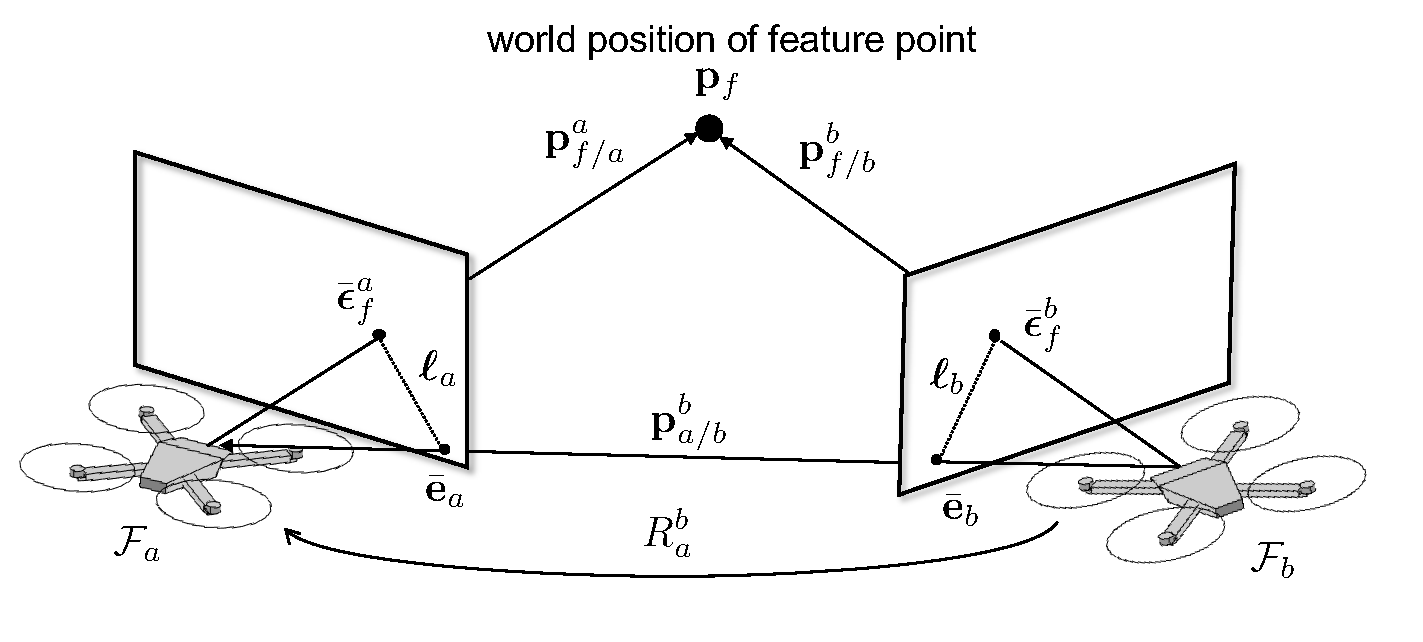
\includegraphics[width=\linewidth]{chap8_scene_reconstruction/figures/epipolar_geometry_quad}
		\caption{Epipolar Geometry}
		\label{fig:epipolar_geometry}
	\end{figure}
The relationship between $\pbf_{f/a}^a$ and $\pbf_{f/b}^b$ is given by
\begin{equation}\label{eq:scene_geometric_relation}
\pbf_{f/b}^b = R_a^b \pbf_{f/a}^a + \pbf_{a/b}^b,
\end{equation}
as shown in Figure~\ref{fig:epipolar_geometry}.  Multiplying both sides of  Equation~\eqref{eq:scene_geometric_relation} on the left by $\ss{\pbf_{a/b}^b}$ gives
\[
\ss{\pbf_{a/b}^b} \pbf_{f/b}^b = \ss{\pbf_{a/b}^b} R_a^b \pbf_{f/a}^a,
\]
where we have used the fact that $\ss{\pbf_{a/b}^b}\pbf_{a/b}^b = \pbf_{a/b}^b \times \pbf_{a/b}^b = 0$. Since $\ss{\pbf_{a/b}^b} \pbf_{f/b}^b = \pbf_{a/b}^b \times \pbf_{f/b}^b$ must be orthogonal to $\pbf_{f/b}^b$ we have that 
\begin{equation}\label{eq:scene_epipolar_1}
\pbf_{f/b}^{b\top} \ss{\pbf_{a/b}^b} R_a^b \pbf_{f/a}^a = 0.
\end{equation}
Dividing Equation~\eqref{eq:scene_epipolar_1} by the norm of $\pbf_{a/b}^b$, and defining
\[
\nbf_{a/b}^b\defeq \frac{\pbf_{a/b}^b}{\norm{\pbf_{a/b}^b}}
\]
gives
\begin{equation}\label{eq:scene_epipolar_2}
\pbf_{f/b}^{b\top} \ss{\nbf_{a/b}^b} R_a^b \pbf_{f/a}^a = 0.
\end{equation}
The matrix 
\begin{equation}\label{eq:scene_essential_matrix}
E = \ss{\nbf_{a/b}^b} R_a^b
\end{equation}
is called the essential matrix, and is completely defined by the relative pose $(R_a^b, \pbf_{a/b}^b)$.  
\begin{theorem}
	Given the geometry shown in Figure~\ref{fig:epipolar_geometry} with relative pose $(R_a^b, \pbf_{a/b}^b)$, and the associated essential matrix given in Equation~\eqref{eq:essential_matrix}.  Every pair of matching feature points  $(\bar{\epsilonbf}_{f/a}^a, \bar{\epsilonbf}_{f/b}^b)$ in frames $a$ and $b$, expressed in normalized (calibrated) coordinates satisfies the so-called {\em epipolar constraint}
	\begin{equation}\label{eq:scene_epipolar_3}
	\bar{\epsilonbf}_{f/b}^{b\top} ~E~ \bar{\epsilonbf}_{f/a}^a = 0.
	\end{equation}
\end{theorem}
\begin{proof}
The normalized pixel coordinates of the feature point projected on to image $a$ and image $b$ satisfy
\begin{align*}
\lambda_a \bar{\epsilonbf}_{f/a}^a &= \pbf_{f/a}^a \\
\lambda_b \bar{\epsilonbf}_{f/b}^b &= \pbf_{f/b}^b,
\end{align*}
where $\lambda_a$ and $\lambda_b$ are the distances to the feature point along the optical axes in frame $a$ and $b$, respectively.  Substituting into Equation~\eqref{eq:scene_epipolar_2} gives
\begin{equation}\label{eq:scene_epipolar_3}
\bar{\epsilonbf}_{f/b}^{b\top} E \bar{\epsilonbf}_{f/a}^a = 0.
\end{equation}
\end{proof}

There is a related result for uncalibrated coordinates.
\begin{theorem}
	Define the {\em fundamental matrix} as
	\begin{equation}\label{eq:scene_fundamental_matrix}
	F = K_c^{-\top} E K_c^{-1},
	\end{equation}
	where $K_c$ is the camera calibration matrix.  Then every set of matching pixels $(\bar{\mbf}_{f/a}^a, \bar{\mbf}_{f/b}^b)$ in homogeneous (uncalibrated) coordinates satisfies
	\begin{equation}\label{eq:scene_epipolar_4}
	\bar{\mbf}_{f/b}^{b\top} ~F~ \bar{\mbf}_{f/a}^a = 0.
	\end{equation}
\end{theorem}
\begin{proof}
	Follows directly from Equation~\eqref{eq:scene_epipolar_3} and the fact that $\bar{\epsilonbf} = K_c^{-1} \bar{\mbf}$.
\end{proof}

The essential matrix invokes several interesting geometrical relationships.  For example, consider the relationship
\begin{align*}
\ellbf_a &= E^\top \bar{\epsilonbf}^b\\
	&= R_a^{b\top} \ss{\nbf_{a/b}^b}^\top \bar{\epsilonbf}^b \\
	&= R_b^a (\bar{\epsilonbf}^b \times \nbf_{a/b}^b),
\end{align*}
from which it is clear that $\ellbf_a$ is a vector (expressed in frame $a$) that is perpendicular to both $\bar{\epsilonbf}^b$ and $\nbf_{a/b}^b$.  Therefore $\ellbf_a$ is perpendicular to the epipolar plane containing $\pbf_{a/b}$, $\pbf_{f/a}$ and $\pbf_{f/b}$.  Since $\ellbf_a$ is in homogenous coordinates, it defines the line in image $a$ where the epipolar plane intersects image $a$.  
%
Similarly, consider the relationship
\begin{align*}
\ell_b &= E \bar{\epsilonbf}^a \\
       &= \ss{\nbf_{a/b}^b}R_a^b \bar{\epsilonbf}^a \\
       &= R_a^b R_a^{b\top} \ss{\nbf_{a/b}^b}R_a^b \bar{\epsilonbf}^a \\
       &= R_a^b \ss{R_a^{b\top}\nbf_{a/b}^b} \bar{\epsilonbf}^a\\
       &= R_a^b \ss{\nbf_{a/b}^a} \bar{\epsilonbf}^a \\
       &= R_a^b (\nbf_{a/b}^a \cross \bar{\epsilonbf}^a),
\end{align*}
from which it is clear that $\ell_b$ is a vector (expressed in frame $b$) that is perpendicular to both $\bar{\epsilonbf}^a$ and $\nbf_{a/b}^a$.  Therefore $\ellbf_b$ is also perpendicular to the epipolar plane containing $\pbf_{a/b}$, $\pbf_{f/a}$ and $\pbf_{f/b}$.  Since $\ellbf_b$ is in homogenous coordinates, it defines the line in image $b$ where the epipolar plane intersects image $b$.  
%
The lines $\ellbf_a$ and $\ellbf_b$ are called the epipolar lines.  

As shown in Figure~\ref{fig:epipolar_geometry}, the vector $\pbf_{a/b}^b$ intersects the two image planes (typically outside the field-of-view) at the points $\bar{\ebf}_a$ and $\bar{\ebf}_b$ which are called the epipoles.  Since any line in the image can be defined by the cross product of two points on the line, the epipoles are defined by the relationship
\begin{align*}
\ellbf_a &= \bar{\epsilonbf}^a \times \bar{\ebf}^a \\
\ellbf_b &= \bar{\epsilonbf}^b \times \bar{\ebf}^b.
\end{align*}

\rwbcomment{Add:  (1) How to compute $E$ from matching image points. (2) Given $E$, how to fine $R$ and $\nbf$. (3) Other interesting facts about epipolar geometry.}  
	
%-------------------------------------------------------
\subsection{Point Triangulation}
	
	We desire to recover point locations in 3-space given two camera views of the same point. In the ideal case where there is no noise or discretization in pixel coordinates of the imaged point, this can be done using a simple triangulation method. However, consider the case shown in Fig.~\ref{fig:noise}. If there is any noise in homogeneous image coordinates in either of the images, the rays from camera centers through the noisy image coordinates will never intersect, and the epipolar constraint will not be satisfied. A simple way to overcome this issue is to pick the midpoint of the line segment of minimum length that connects the two rays as the 3D point. However, this method of error minimization is not projective-invariant \cite{Hartley2004}. A more suitable method is presented in Section \ref{sec:mle_triang}.
	
	\begin{figure}
		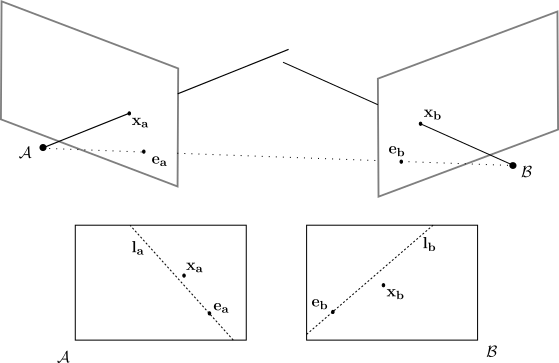
\includegraphics[width=\linewidth]{chap8_scene_reconstruction/figures/epipolar_noise}
		\caption{Effect of noise on epipolar geometry.}
		\label{fig:noise}
	\end{figure}
	
%--------------------------------------------------------	
\subsection{Naive Point Triangulation}
\label{sec:naive}
In this section we will describe a simple method for point triangulation when the relative pose $(R_a^b, \pbf_{a/b}^b)$ are known.
\begin{theorem}
	Suppose that the relative pose $(R_a^b, \pbf_{a/b}^b)$ is known, and that the normalized (calibrated) pixel coordinates of a feature are known, i.e.,
	\begin{align*}
	\bar{\epsilonbf}_{f/a}^a &= \lambda_a \pbf_{f/a}^a \\
	\bar{\epsilonbf}_{f/b}^b &= \lambda_b \pbf_{f/b}^b.
	\end{align*}
	Then the unknown scales are given by
	\begin{align*}
	\lambda_a &= -\norm{\pbf_{a/b}^b}\frac{(R_a^b\bar{\epsilonbf}_{f/a}^a)^\top \ss{\bar{\epsilonbf}_{f/b}^b} E R_a^{b\top} \bar{\epsilonbf}_{f/b}^b}
	{\norm{\ss{\bar{\epsilonbf}_{f/b}^b}R_a^b\bar{\epsilonbf}_{f/a}^a}},
	\\
	\lambda_b &= \norm{\pbf_{a/b}^b} \frac{\bar{\epsilonbf}_{f/b}^{b\top}\ss{R_a^b\bar{\epsilonbf}_{f/a}^a} E \bar{\epsilonbf}_{f/a}^a}
	{\norm{\ss{R_a^b\bar{\epsilonbf}_{f/a}^a}\bar{\epsilonbf}_{f/b}^b}},
	\end{align*}
	where $E=\ss{\frac{\pbf_{a/b}^b}{\norm{\pbf_{a/b}^b}}}R_a^b$ is the essential matrix.
\end{theorem}
\begin{proof}
	From Equation~\eqref{eq:scene_geometric_relation}  we have
	\[
	\pbf_{f/b}^b = R_a^b \pbf_{f/a}^a + \pbf_{a/b}^b.
	\]
	In terms of calibrated pixel coordinates we have
	\[
	\lambda_b \epsilonbf_{f/b}^b = \lambda_a R_a^b \epsilonbf_{f/a}^a + \pbf_{a/b}^b,
	\]	
	where $\lambda_a$ and $\lambda_b$ are unknown scales.  
	Multiplying both sides by $\ss{R_a^b \epsilonbf_{f/a}^a}$ gives
	\[
	\lambda_b \ss{R_a^b \epsilonbf_{f/a}^a} \epsilonbf_{f/b}^b  = \ss{R_a^b \epsilonbf_{f/a}^a} \pbf_{a/b}^b.
	\]	
	Multiplying booth sides by $(\ss{R_a^b \epsilonbf_{f/a}^a} \epsilonbf_{f/b}^b)^\top$, and solving for the scale $\lambda_b$ gives
	\[
	\lambda_b = \frac{(\ss{R_a^b \epsilonbf_{f/a}^a} \epsilonbf_{f/b}^b)^\top \ss{R_a^b \epsilonbf_{f/a}^a} \pbf_{a/b}^b}{\norm{\ss{R_a^b \epsilonbf_{f/a}^a} \epsilonbf_{f/b}^b}^2}.
	\]
	The numerator can be simplified as
	\begin{align*}
	& (\ss{R_a^b \epsilonbf_{f/a}^a} \epsilonbf_{f/b}^b)^\top \ss{R_a^b \epsilonbf_{f/a}^a} \pbf_{a/b}^b \\
	=& -\epsilonbf_{f/b}^{b\top} \ss{R_a^b \epsilonbf_{f/a}^a}  \ss{R_a^b \epsilonbf_{f/a}^a} \pbf_{a/b}^b \\
	=& \epsilonbf_{f/b}^{b\top} \ss{R_a^b \epsilonbf_{f/a}^a} \ss{\pbf_{a/b}^b} R_a^b \epsilonbf_{f/a}^a  \\
	=& \norm{\pbf_{a/b}^b} \epsilonbf_{f/b}^{b\top} \ss{R_a^b \epsilonbf_{f/a}^a} E \epsilonbf_{f/a}^a.
	\end{align*}
	The formula for $\lambda_a$ is derived similarly.
\end{proof}

\rwbcomment{Revise stuff below to fit notation.}

	Let $\pbf_{f/a}^a$ and $\pbf_{f/b}^b$ be the position vector of a feature in frames $a$ and $b$ respectively.  Then
	\[
	\pbf_{f/b}^b = R_a^b \pbf_{f/a}^a + \pbf_{a/b}^b.
	\]
	In terms of calibrated pixel coordinates we have
	\[
	\lambda_b \epsilonbf_{f/b}^b = \lambda_a R_a^b \epsilonbf_{f/a}^a + \gamma \nbf_{a/b}^b,
	\]	
	where $\lambda_a$, $\lambda_b$, and $\gamma$ are unknown scales.  Multiplying both sides by $\ss{\epsilonbf_{f/b}^b}$ gives
	\begin{align*}
	& \lambda_a \ss{\epsilonbf_{f/b}^b} R_a^b \epsilonbf_{f/a}^a + \gamma \ss{\epsilonbf_{f/b}^b} \nbf_{a/b}^b = 0 \\
	\implies & \begin{pmatrix} \ss{\epsilonbf_{f/b}^b} R_a^b \epsilonbf_{f/a}^a & \ss{\epsilonbf_{f/b}^b} \nbf_{a/b}^b\end{pmatrix}\begin{pmatrix} \lambda_a \\  \gamma \end{pmatrix}  = 0.
	\end{align*}
	
	Suppose not that there are $n$ features tracked between frames $a$ and $b$, and let $\epsilonbf_{f_i/b}^b$ and $\epsilonbf_{f_{i/a}}^a$ be the corresponding feature locations in normalized calibrated pixels.  Then the depth factors $\lambda_{i/a}$ relative to frame $a$ and the depth factor $\gamma$ satisfy
	\[
	M\lambdabf \defeq \begin{pmatrix}
 					  	\ss{\epsilonbf_{f_1/b}^b} R_a^b \epsilonbf_{f_1/a}^a & \mathbf{0} & \cdots & \mathbf{0} & \ss{\epsilonbf_{f_1/b}^b} \nbf_{a/b}^b \\
 					  	\mathbf{0} & \ss{\epsilonbf_{f_2/b}^b} R_a^b \epsilonbf_{f_2/a}^a & \cdots & \mathbf{0} & \ss{\epsilonbf_{f_2/b}^b} \nbf_{a/b}^b \\
 					  	\vdots & \vdots & \ddots & \vdots & \vdots \\
 					  	\mathbf{0} & \mathbf{0} & \cdots & \ss{\epsilonbf_{f_n/b}^b} R_a^b \epsilonbf_{f_n/a}^a & \ss{\epsilonbf_{f_n/b}^b} \nbf_{a/b}^b
 					  \end{pmatrix}
 					  \begin{pmatrix} \lambda_{1/a} \\ \lambda_{2/a} \\ \vdots \\ \lambda_{n/a} \\ \gamma \end{pmatrix} = \mathbf{0}.
	\]
	Therefore, the unknown scale factors $\lambdabf$ are in the null space of the $3n\times(n+1)$ matrix $M$.  Let
	\[
		M = \begin{pmatrix}U_1 & U_2 \end{pmatrix}\begin{pmatrix}\Sigma & 0 \\ 0 & 0 \end{pmatrix} \begin{pmatrix} V_1^\top \\ V_2^\top \end{pmatrix}
	\]
	be the singular value decomposition of $M$, then $\lambdabf = V_2\in\mathbb{R}^{(n+1)\times 1}$.  Note that any scaled version of $V_2$ is also a solution.  Therefore, to use this method we require one of the parameters $\lambda_{1/a}, \dots, \lambda_{n/a}, \gamma$ to be known.  If for example, the translation $\gamma$ is known via, e.g., IMU integration, then $V_2$ is scaled so that its last element equals $\gamma$, and the rest of the scale factors are recovered.
		
	\begin{theorem}
		The matrix $M$ defined above has a null space with dimension one if and only iff the pixel pairs $(\epsilonbf_{f_i/b}^b, \epsilonbf_{f_{i/a}}^a)$ satisfy the epipolar constraint, and the originating point $\mathbf{p}_f$ does not lie along the epipolar baseline.
	\end{theorem}
	
	\begin{proof}
		If $(\epsilonbf_{f_i/b}^b, \epsilonbf_{f_{i/a}}^a)$ do not satisfy the epipolar constraint, i.e.
		\[
		\epsilonbf_{f_{i/b}}^{b\top} E_{a}^b \epsilonbf_{f_{i/a}}^a = \mu, 
		\]
		where $\mu \neq 0$.  It is clear that the first $n$ columns of $M$ are linearly independent.  Therefore $M$ is at least rank $n$, and will be rank $n+1$ iff the last column can be written as linear combination of the first $n$ columns.  		
		 Considering only rows associated with the $i^{th}$ pixel pair,  there must exist a non-zero constant $c$ such that 
		\[
		c \ss{\epsilonbf_{f_{i/b}}^b} R_a^b \epsilonbf_{{f_i}/a}^a = \ss{\epsilonbf_{f_{i/b}}^b} \nbf_{a/b}^b.
		\]
		Multiplying both sides by $\nbf_{a/b}^{b\top}$ gives
		\begin{align*}
		&c \nbf_{a/b}^{b\top} \ss{\epsilonbf_{f_i/b}^b} R_a^b \epsilonbf_{f_{i/a}}^a = \nbf_{a/b}^{b\top}\ss{\epsilonbf_{f_i/b}^b} \nbf_{a/b}^b \\
		\implies & = -c \epsilonbf_{f_i/b}^{b\top} \ss{\nbf_{a/b}^{b}} R_a^b \epsilonbf_{f_{i/a}}^a = 0 \\
		&\quad = -c \epsilonbf_{f_i/b}^{b\top} E_a^b \epsilonbf_{f_{i/a}}^a = 0  \\
		&\quad = -c \mu = 0.
		\end{align*}
		Therefore, if the epipolar constraint is not satisfied for the $i^{th}$, then $c$ must be 0 to satisfy this relationship. 
		If $c=0$, then we must have that
		\[
		\ss{\epsilonbf_{f_i/b}^b} \nbf_{a/b}^b = 0
		\]
		which is true only when $\epsilonbf_{f_i/b}^b$ is imaged at the epipole in frame $b$. 		
	\end{proof}
		
	
%--------------------------------------------------------	
	\subsection{Point Triangulation Using Maximum Likelihood Estimation}
	\label{sec:mle_triang}
	
	\rwbcomment{Revise to fit notation.}
	
	The solution obtained in section \ref{sec:naive} assumed that the normalized image points $\mathbf{\bar{x}_a}$ and $\mathbf{\bar{x}_b}$ satisfy the epipolar constraint. However, image coordinates are likely to be subject to noise caused by imperfect feature matching, discretization, imperfect camera models, inaccurate distortion correction, etc. This noise causes the epipolar constraint to not be satisfied. 
	
	We seek to obtain a new point correspondence $\mathbf{\hat{\bar{x}}_a}$, $\mathbf{\hat{\bar{x}}_b}$ that minimizes the distance between measured and new points such that the epipolar constraint is satisfied, as shown in Fig. \ref{fig:noise_corr}. This results in the problem
	\begin{equation}
	\min_{\mathbf{\hat{\bar{x}}_a},\mathbf{\hat{\bar{x}}_b}} \quad d(\mathbf{\bar{x}_a}, \mathbf{\hat{\bar{x}}_a})^2 + d(\mathbf{\bar{x}_b}, \mathbf{\hat{\bar{x}}_b})^2 \quad \text{s.t.} \quad \mathbf{\hat{\bar{x}}_b}^\top E_{ab} \mathbf{\hat{\bar{x}}_a} = 0,
	\label{eq:cost}
	\end{equation}
	where $d(*,*)$ is the 2-norm between the two points. 
	
	This problem can be solved using any iterative minimization strategy. However, section 12.5 of \cite{Hartley2004} presents an analytical solution that involves finding the roots of a six-degree polynomial. Additionally, section 12.4 presents the solution to the first order approximation of Eq. \ref{eq:cost} that can be used so long as the error in image coordinates is around 1 pixel.
	
	After a solution to Eq. \ref{eq:cost} is obtained, the method presented in section \ref{sec:naive} can be used to obtain the triangulation for $\mathbf{X_a}$.
	
	\begin{figure}
		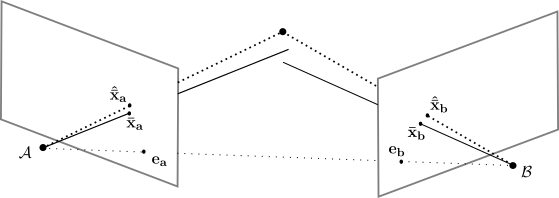
\includegraphics[width=\linewidth]{chap8_scene_reconstruction/figures/epipolar_noise_corr}
		\caption{Maximum likelihood estimate of image correspondence that satisfies the epipolar constraint.}
		\label{fig:noise_corr}
	\end{figure}



%------------------------------------------------
\section{Simple point reconstruction methods}
\label{sec:point_reconstruction}

The point reconstruction problem is depicted graphically in Figure~\ref{fig:scene_reconstruction}, where the airc

\begin{figure}[h]
	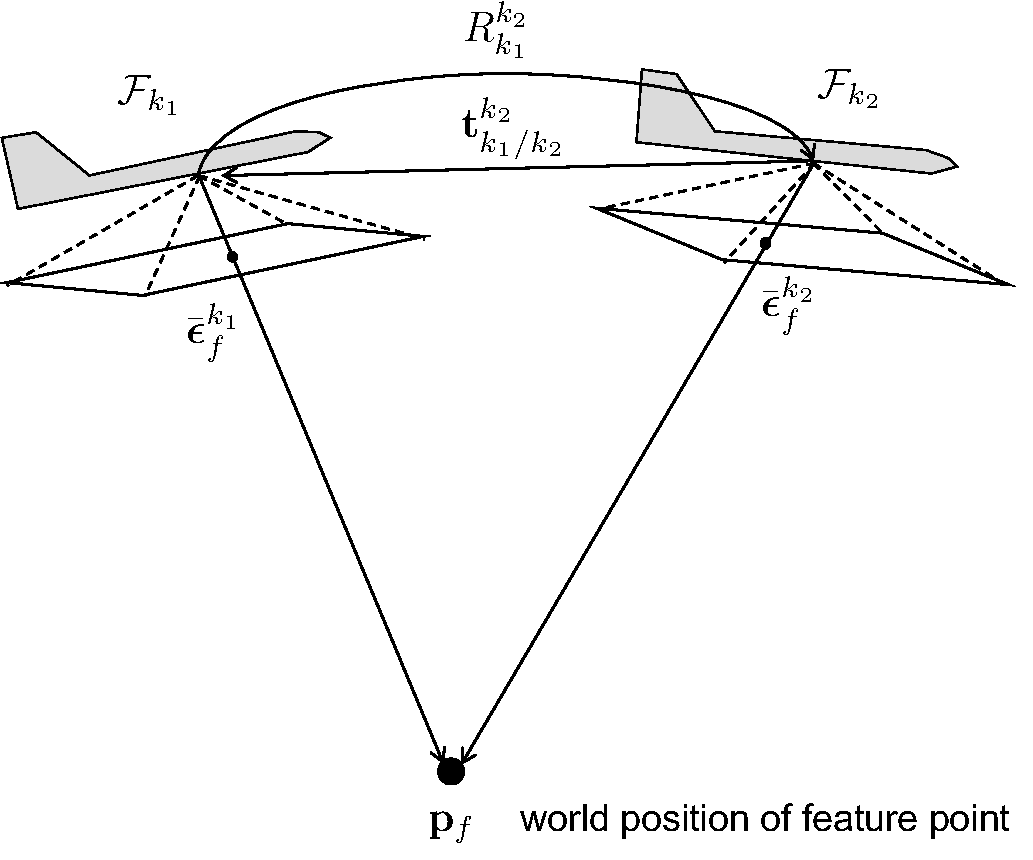
\includegraphics[width=0.8\linewidth]{chap8_scene_reconstruction/figures/point_reconstruction}
	\caption{The point reconstruction problem.}
	\label{fig:point_reconstruction}
\end{figure}

%------------------------------------------------
\section{Visual Inertial Odometry }
\label{sec:vio}

%----------------------------
\subsection{Error State EKF}

Sometimes called indirect Kalman filter, or multiplicative Kalman filter.

\begin{figure}[h]
	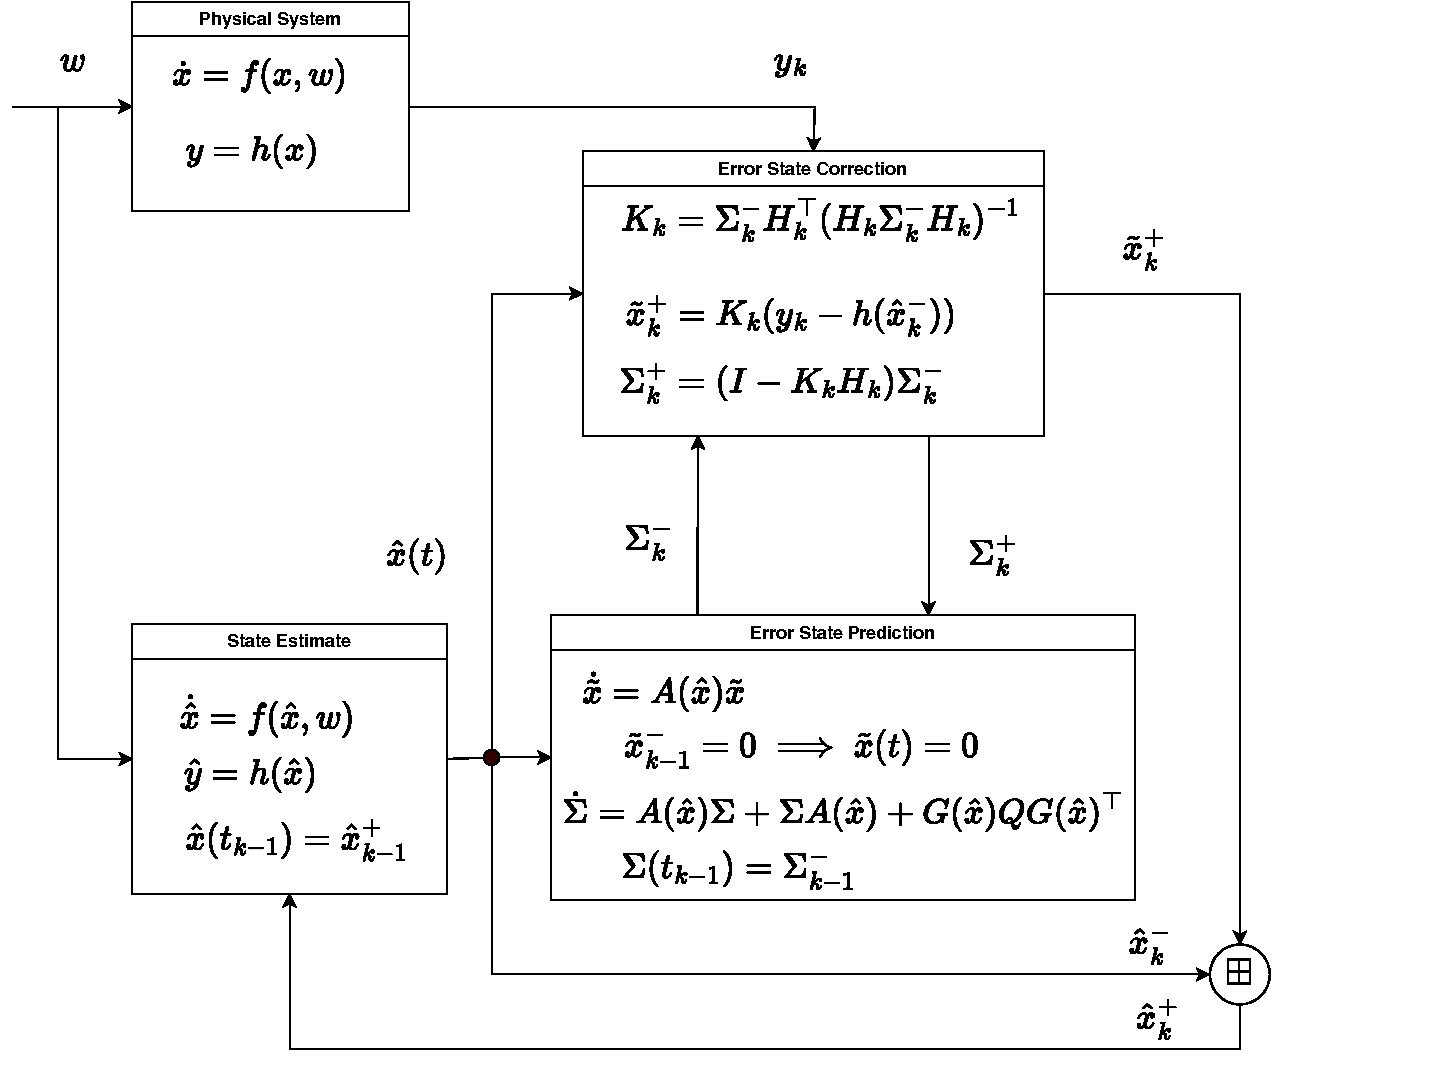
\includegraphics[width=0.99\linewidth]{chap8_scene_reconstruction/figures/indirectEKF}
	\caption{Block diagram for the error state extended Kalman filter (ESEKF).}
	\label{fig:indirectEKF}
\end{figure}

The algorithm is implemented as follows:
\par\noindent{\bf Between Measurements}
	\begin{itemize}
		\item Propagate the state estimate for $t\in[t_{k-1}, t_k)$:
			\[ 
			\dot{\hat{x}} = f(\hat{x}, w),
			\]
			with initial conditions $\hat{x}(t_{k-1}) = \hat{x}_{k-1}^+$.
			The solution at time $t=t_k$ is $\hat{x}_k^-$.
		\item The error state is propagated as $\tilde{x}(t)=0$. ($\dot{\tilde{x}}=A\tilde{x}$ with initial conditions $\tilde{x}(t_{k-1})=0$)
		\item Propagate the error covariance for $t\in[t_{k-1}, t_k)$:
			\[
			\dot{\Sigma} = A\left(\hat{x}(t), w(t)\right)\Sigma + \Sigma A\left(\hat{x}(t), w(t)\right)) + G\left(\hat{x}(t), w(t)\right)) Q G\left(\hat{x}(t), w(t)\right))^\top
			\]
			with initial condition $\Sigma(t_{k-1}) = \Sigma_{k-1}^+$. 
			The solution at time $t=t_k$ is $\Sigma_k^-$.
	\end{itemize}
\par\noindent{\bf At the Measurement of sensor $s$:}
	\begin{itemize}
		\item Compute the Kalman gain:
			\[ 
			K_s = \Sigma_k^- H_s^\top(\hat{x}_k^-)\left(H_s(\hat{x}_k^-)\Sigma_k^-H_s^\top(\hat{x}_k^-)+R_k\right)^{-1}
			\]
		\item Compute the predicted measurement $\hat{y}_s = h_s(\hat{x}_k^-)$
		\item Update the error state:
			\[
			\tilde{x}_k^+ = K_x \left( y_s(t_k) - \hat{y}_s \right)
			\]
		\item Update the error covariance:
			\[
			\Sigma_k^+ = \left(I-K_s H_s(\hat{x}_k^-)\right)\Sigma_k^-
			\]
		\item Update the state estimate:
			\[
			\hat{x}_k^+ = \hat{x}_k^- \boxplus \tilde{x}_k^+
			\]
	\end{itemize}



%----------------------------
\subsection{Almost-Invariant EKF for VIO}

In this section we outline a method for combining visual and IMU measurements to estimate the position of the vehicle as well as the position of features in the environment, assuming no IMU biases.  We will assume that the camera moves according to \eqref{eq:camera_motion_p}--\eqref{eq:camera_motion_R} which we repeat here for convenience
\begin{align*}
\dot{\pbf}_{b/i}^i &= \vbf_{b/i}^i   \\
\dot{\vbf}_{b/i}^i &= \gbf^i \ebf_3 + R_b^i (\abf_{b/i}^b-\bbf_a),  \\
\dot{R}_b^i &= R_b^i \ss{\omegabf_{b/i}^b-\bbf_\omega} \\
\dot{\bbf}_a &= 0 \\
\dot{\bbf}_\omega &= 0 \\
\dot{\ellbf}_1 &= 0 \\
&\vdots \\ 
\dot{\ellbf}_N &= 0,
\end{align*}
where we assumed that the body and camera frames are aligned, and where we have assumed a set of $N$ stationary landmarks in the environment $\{\ellbf_i\}_{i=1}^N$, where $\ellbf_i\in\mathbb{R}^3$.

In this section we derive an error state extended Kalman filter that uses the state prediction equations
\begin{align*}
\dot{\hat{\pbf}}_{b/i}^i &= \hat{\vbf}_{b/i}^i   \\
\dot{\hat{\vbf}}_{b/i}^i &= \gbf^i \ebf_3 + \hat{R}_b^i (\abf_{b/i}^b -\hat{\bbf}_a),  \\
\dot{\hat{R}}_b^i &= \hat{R}_b^i \ss{\omegabf_{b/i}^b-\hat{\bbf}_\omega} \\
\dot{\hat{\bbf}}_a &= 0 \\
\dot{\hat{\bbf}}_\omega &= 0 \\
\dot{\hat{\ellbf}}_i &= 0.
\end{align*}

Following the development of the Invariant Kalman Filter~\cite{}, we define the errors in the inertial frame as
\begin{align*}
    \tilde{\pbf} &= \hat{\pbf}^{\hat{i}}-\hat{R}_b^{\hat{i}}R_b^{i\top} \pbf^i \\
    \tilde{\vbf} &= \hat{\vbf}^{\hat{i}}-\hat{R}_b^{\hat{i}}R_b^{i\top} \vbf^i \\
    \tilde{\rbf} &= \log(\hat{R}_b^{\hat{i}} R_b^{i\top})^\vee \\
    \tilde{\bbf}_a &= \hat{\bbf}_a - \bbf_a \\
	\tilde{\bbf}_\omega &= \hat{\bbf}_\omega - \bbf_\omega \\
    \tilde{\ellbf}_i &= \hat{\ellbf}_i^{\hat{i}}-\hat{R}_b^{\hat{i}}R_b^{i\top} \ellbf_i^i
\end{align*}

Differentiating the position errors gives
\begin{align*}
    \dot{\tilde{\pbf}} &= \dot{\hat{\pbf}}^{\hat{i}}-\dot{\hat{R}}_b^{\hat{i}} R_b^{i\top}\pbf^i - \hat{R}_b^{\hat{i}}\frac{d}{dt}(R_b^{i\top}) \pbf^i - \hat{R}_b^{\hat{i}}R_b^{i\top} \dot{\pbf}^i \\
     &= \hat{\vbf}^{\hat{i}} - \hat{R}_b^{\hat{i}}\ss{\omegabf^b-\hat{\bbf}_\omega} R_b^{i\top} \pbf^i + \hat{R}_b^{\hat{i}} R_b^{i\top} R_b^i\ss{\omega^b-\bbf_\omega} R_b^{i\top} \pbf^i - \hat{R}_b^{\hat{i}} R_b^{i\top} \vbf^i \\
     &= \hat{\vbf}^{\hat{i}} - \hat{R}_b^{\hat{i}}R^{i\top} \vbf^i   - \hat{R}_b^{\hat{i}}\ss{\tilde{\bbf}_\omega} R_b^{i\top} \pbf^i \\ 
    &= \tilde{\vbf}^{\hat{i}}  - \ss{\hat{R}_b^{\hat{i}}\tilde{\bbf}_\omega}\hat{R}_b^{\hat{i}}R^{i\top} (\hat{R}_b^{\hat{i}}R^{i\top})^\top(\hat{\pbf}-\tilde{\pbf}) \\
    &= \tilde{\vbf}^{\hat{i}}  - \ss{\hat{R}_b^{\hat{i}}\tilde{\bbf}_\omega}\hat{\pbf} + \ss{\hat{R}_b^{\hat{i}}\tilde{\bbf}_\omega}\tilde{\pbf} \\   
    &\approx \tilde{\vbf}^{\hat{i}}  + \ss{\hat{\pbf}} \hat{R}_b^{\hat{i}}\tilde{\bbf}_\omega \\     
\end{align*}
Differentiating the velocity errors gives
\begin{align*}
    \dot{\tilde{\vbf}}^{\hat{i}} &= \dot{\hat{\vbf}}^{\hat{i}}-\dot{\hat{R}}_b^{\hat{i}} R_b^{i\top} \vbf^i - \hat{R}_b^{\hat{i}} \frac{d}{dt}(R_b^{i\top}) \vbf^i -\hat{R}_b^{\hat{i}} R_b^{i\top} \dot{\vbf}^i \\
    &= (\gbf^i + \hat{R}_b^{\hat{i}} (\abf^b+\hat{\bbf}_a)-\hat{R}_b^{\hat{i}} \ss{\omegabf^b-\hat{\bbf}_\omega} R_b^{i\top} \vbf^i - \hat{R}_b^{\hat{i}} R_b^{i\top} R_b^i \ss{\omegabf^b-\bbf_\omega} R_b^{i\top} \vbf^i -\hat{R}_b^{\hat{i}} R_b^{i\top}(\gbf^i + R_b^i (\abf^b-\bbf_a) \\
    &= (I-\hat{R}_b^{\hat{i}}R_b^{i\top})\gbf^i + \hat{R}_b^{\hat{i}}\tilde{\bbf}_a - \hat{R}_b^{\hat{i}}\ss{\tilde{\bbf}_\omega} R_b^{i\top} \vbf^i  \\
    &\approx (I - \exp(\ss{\tilde{\rbf}}) ) \gbf^i + \hat{R}_b^{\hat{i}}\tilde{\bbf}_a - \ss{\hat{R}_b^{\hat{i}}\tilde{\bbf}_\omega} \hat{R}_b^{\hat{i}} R_b^{i\top} (\hat{R}_b^{\hat{i}} R_b^{i\top})^\top ( \hat{\vbf}^i - \tilde{\vbf})  \\
    &\approx -\ss{\tilde{\rbf}} \gbf^i + \hat{R}_b^{\hat{i}}\tilde{\bbf}_a - \ss{\hat{R}_b^{\hat{i}}\tilde{\bbf}_\omega}\hat{\vbf}^i  \\
    &= \ss{\gbf^i} \tilde{\rbf} + \hat{R}_b^{\hat{i}}\tilde{\bbf}_a + \ss{\hat{\vbf}^i} \hat{R}_b^{\hat{i}}\tilde{\bbf}_\omega.
\end{align*} 
For the evolution of the attitude error we use the fact that
\[
\frac{d}{dt}\exp(\ss{\tilde{\rbf}}) 
    \approx \frac{d}{dt}(I + \ss{\tilde{\rbf}}) = \ss{\dot{\tilde{\rbf}}},
\]
to get that 
\begin{align*}
    \dot{\tilde{\rbf}}
        &= \left(\dot{\hat{R}}_b^i R_b^{i\top} + \hat{R}_b^i\frac{d}{dt}(R_b^{i\top})\right)^\vee \\
        &= \left(\hat{R}_b^i\ss{\omegabf^b-\hat{\bbf}_\omega} R_b^{i\top} - \hat{R}_b^iR_b^{i\top} R_b^i \ss{\omegabf^b-\bbf_\omega} R_b^{i\top}\right)^\vee \\
        &= -\left(\hat{R}_b^i\ss{\hat{\bbf}_\omega} R_b^{i\top} + \hat{R}_b^i \ss{\bbf_\omega} R_b^{i\top}\right)^\vee \\
        &= -\left(\ss{\hat{R}_b^i\tilde{\bbf}_\omega} \hat{R}_b^i R_b^{i\top}\right)^\vee \\        
        &\approx -\left(\ss{\hat{R}_b^i\tilde{\bbf}_\omega} (I + \ss{\tilde{\rbf}})\right)^\vee \\
        &\approx -\left(\ss{\hat{R}_b^i\tilde{\bbf}_\omega} \right)^\vee \\
        &= \hat{R}_b^i\tilde{\bbf}_\omega
\end{align*}
The evolution of a landmark error is given by
\begin{align*}
    \dot{\tilde{\ellbf}} &= \dot{\hat{\ellbf}}^{\hat{i}}-\dot{\hat{R}}_b^{\hat{i}} R_b^{i\top}\ellbf^i - \hat{R}_b^{\hat{i}}\frac{d}{dt}(R_b^{i\top}) \ellbf^i - \hat{R}_b^{\hat{i}}R_b^{i\top} \dot{\ellbf}^i \\
     &=  -\hat{R}_b^{\hat{i}}\ss{\omegabf^b-\hat{\bbf}_\omega} R_b^{i\top} \ellbf^i + \hat{R}_b^{\hat{i}} R_b^{i\top} R_b^i\ss{\omega^b-\bbf_\omega} R_b^{i\top} \ellbf^i  \\
     &=  \hat{R}_b^{\hat{i}}\ss{\tilde{\bbf}_\omega} R_b^{i\top} \ellbf^i  \\
     &=  \ss{\hat{R}_b^{\hat{i}}\tilde{\bbf}_\omega} \hat{R}_b^{\hat{i}}R_b^{i\top} (\hat{R}_b^{\hat{i}}R_b^{i\top})^\top (\hat{\ellbf}^i - \tilde{\ellbf})  \\
     &\approx  \ss{\hat{R}_b^{\hat{i}}\tilde{\bbf}_\omega} \hat{\ellbf}^i  \\
     &\approx  -\ss{\hat{\ellbf}^i} \hat{R}_b^{\hat{i}} \tilde{\bbf}_\omega.
\end{align*}
Therefore, the error state satisfies
\[
\begin{pmatrix} 
	\dot{\tilde{\pbf}}^{\hat{i}} \\ 
	\dot{\tilde{\vbf}}^{\hat{i}} \\ 
	\dot{\tilde{\rbf}} \\ 
	\dot{\tilde{\bbf}}_a \\ 
	\dot{\tilde{\bbf}}_\omega \\  
	\dot{\tilde{\ellbf}}_1 \\ 
	\vdots \\ 
	\dot{\tilde{\ellbf}}_N 
\end{pmatrix}
    = \begin{pmatrix} 0 & I & 0 & 0 & \ss{\hat{\pbf}}\hat{R}_b^{\hat{i}} & 0 & \dots & 0 \\ 
                      0 & 0 & -\ss{\gbf^i} & \hat{R}_b^{\hat{i}} & \ss{\hat{\vbf}^i} \hat{R}_b^{\hat{i}} & 0 & \dots & 0 \\ 
                      0 & 0 & 0 & 0 & \hat{R}_b^{\hat{i}} & 0 & \dots & 0 \\ 
                      0 & 0 & 0 & 0 & 0 & 0 & \dots & 0 \\
                      0 & 0 & 0 & 0 & 0 & 0 & \dots & 0 \\
                      0 & 0 & 0 & 0 & -\ss{\hat{\ellbf}_1^i}\hat{R}_b^{\hat{i}} & 0 & \dots & 0 \\
                      \vdots &  &  & & &  & \dots & \vdots \\ 
                      0 & 0 & 0 & 0 & -\ss{\hat{\ellbf}_N^i}\hat{R}_b^{\hat{i}} & 0 & \dots & 0 
      \end{pmatrix}
      \begin{pmatrix} 
      	\tilde{\pbf}^{\hat{i}} \\ 
      	\tilde{\vbf}^{\hat{i}} \\ 
      	\tilde{\rbf}_r \\ 
      	\tilde{\bbf}_a \\ 
      	\tilde{\bbf}_\omega \\ 
      	\tilde{\ellbf}_1 \\ 
      	\vdots \\ 
      	\tilde{\ellbf}_N 
      \end{pmatrix}.
\]

For the measurement update, we assume that at each sample we observe a subset of the landmarks through the camera.  Therefore, if the $j^{th}$ landmark is observed, then the associated measurement model is
\[
\epsilonbf_j = h(x) \triangleq \pi\left(R_b^{i\top} (\ellbf_j^i - \pbf^i)\right),
\]
where $\pi:\mathbb{R}^3\to\mathbb{R}^2$ is the projection operator from an inertial vector relative to the camera frame to calibrated pixel locations via
\[
\pi((x, y, z)^\top) \triangleq \begin{pmatrix} \frac{x}{z} \\ \frac{y}{z} \end{pmatrix}.
\]
Expressing the measurement in error states gives
\begin{align*}
    \epsilonbf_j &= \pi\left(R_b^{i\top} (\ellbf^i - \pbf^i)\right) \\
      &= \pi\left(R_b^{i\top} \left( (\hat{R}_b^{\hat{i}} R_b^{i\top})^\top (\hat{\ellbf}_j^i - \tilde{\ellbf}_j) - (\hat{R}_b^{\hat{i}} R_b^{i\top})^\top (\hat{\pbf}^{\hat{i}} - \tilde{\pbf}^{\hat{i}})\right) \right) \\
      &= \pi\left(\hat{R}_b^{\hat{i}\top} (\hat{\ellbf}_j - \hat{\pbf}^{\hat{i}}) + \hat{R}_b^{\hat{i}\top} (\tilde{\pbf}-\tilde{\ellbf}_j) \right) \\
      &\approx \pi\left(\hat{\zbf}_j\right) + \frac{\partial\pi}{\partial \zbf}\Big|_{\zbf=\hat{\zbf}_j} \hat{R}_b^{\hat{i}\top} (\tilde{\pbf}-\tilde{\ellbf}_j) ,
\end{align*}
where $\hat{\zbf}_j \triangleq \hat{R}_b^{\hat{i}\top} (\hat{\ellbf}_j - \hat{\pbf}^{\hat{i}})$, and
\[
\frac{\partial\pi}{\partial\zbf}((p_x, p_y, p_z)^\top) = \begin{pmatrix} \frac{1}{p_z} & 0 & -\frac{p_x}{p_z^2} \\ 0 & \frac{1}{p_y} & -\frac{p_y}{p_z^2} \end{pmatrix}.
\]
Defining the matrix
\[
\Pi_j \triangleq \frac{\partial\pi}{\partial \zbf}\Big|_{\zbf=\hat{\zbf}_j},
\]
and letting $\tilde{\epsilonbf}_j = \hat{\epsilonbf}_j - \epsilonbf_j$, 
the output equation can be expressed as
\[
\tilde{\epsilonbf}_j 
    = \begin{pmatrix} 
    	-\Pi_j \hat{R}_b^{\hat{i}\top} & 0 & 0 & 0 & 0 & \dots & \Pi_j\hat{R}_b^{\hat{i}\top} & \dots 
      \end{pmatrix}
      \begin{pmatrix} 
      	\tilde{\pbf}^{\hat{i}} \\ 
      	\tilde{\vbf}^{\hat{i}} \\ 
      	\tilde{\rbf}_r \\ 
      	\tilde{\bbf}_a \\ 
      	\tilde{\bbf}_\omega \\ 
      	\vdots \\
      	\tilde{\ellbf}_j \\ 
      	\vdots 
      \end{pmatrix}.
\]



%------------------------------------------------
\clearpage
\section{Inverse Depth Parametrization for Monocular SLAM, TRO, 2008}
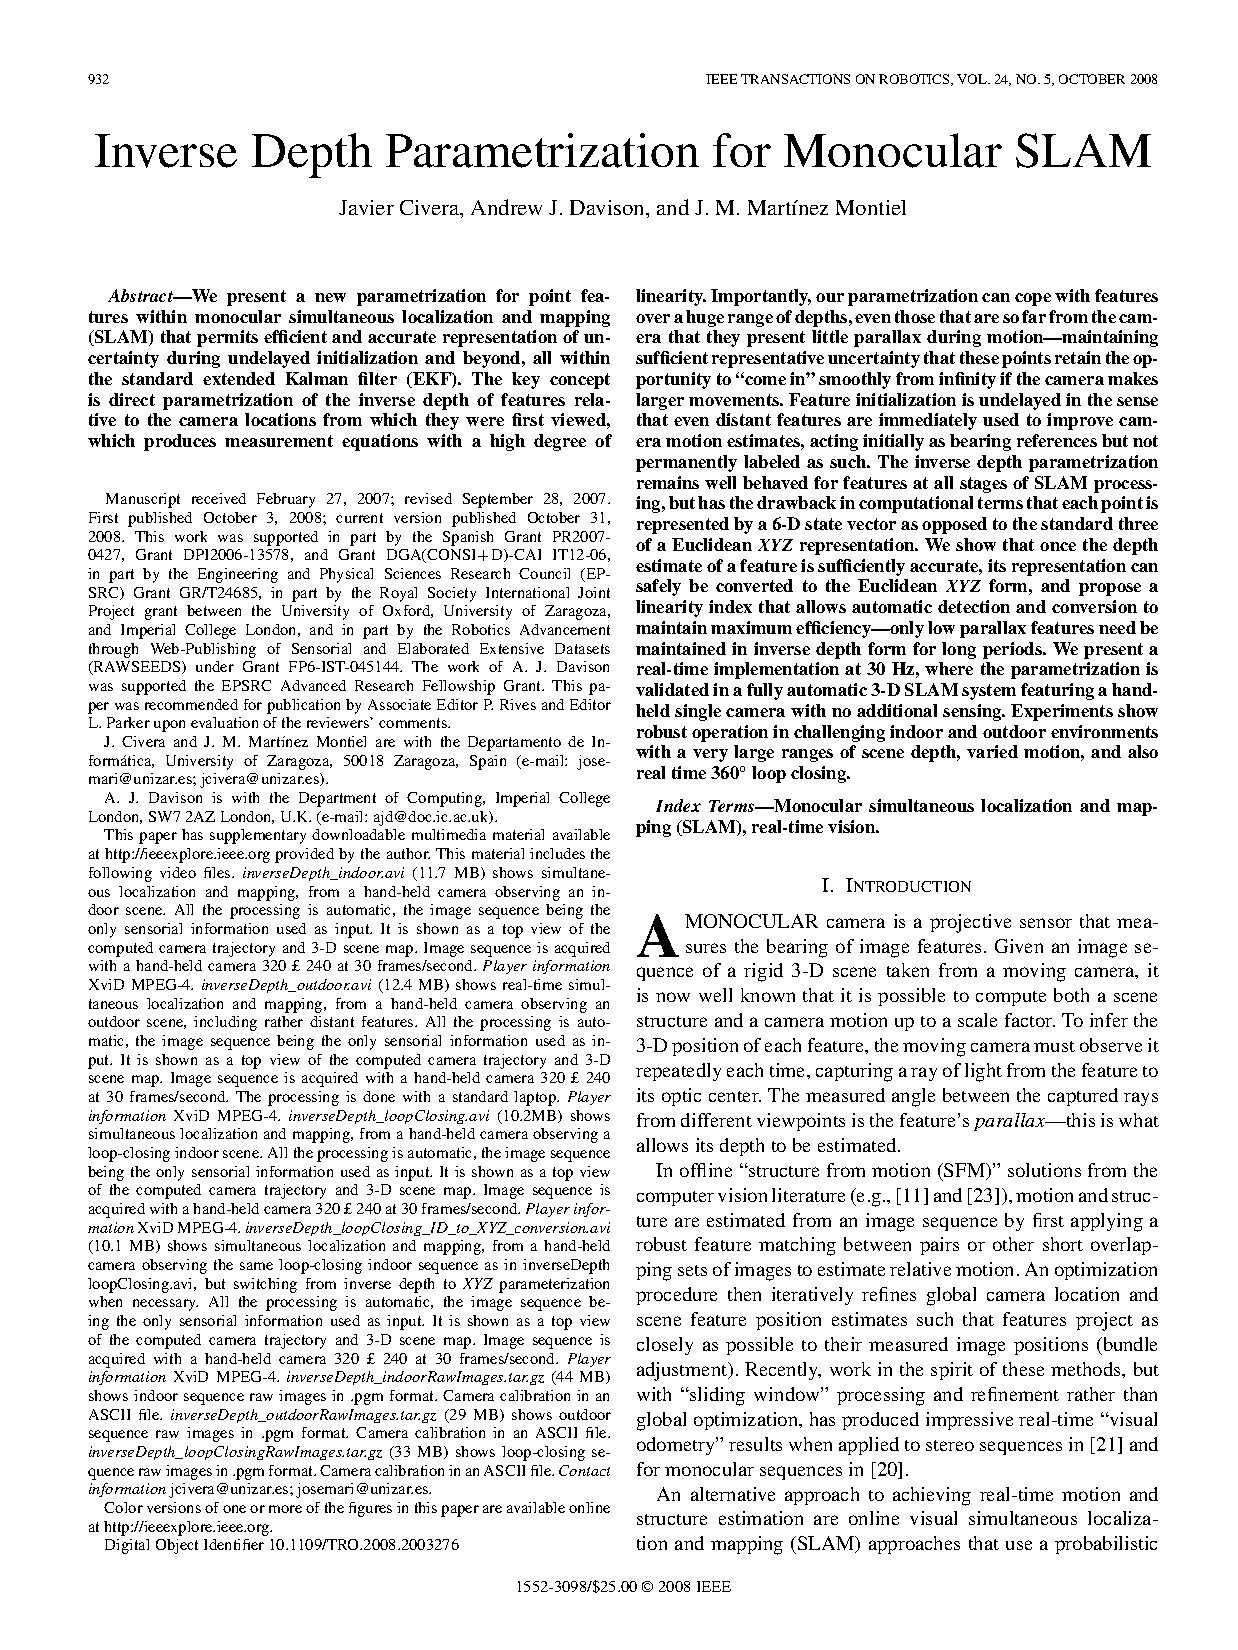
\includepdf[pages=-,scale=.8,pagecommand={}]{chap8_scene_reconstruction/papers/CiveraDavisonMartinez08.pdf}

%------------------------------------------------
\clearpage
\section{Visual Inertial Odometry:  Robust Visual Inertial Odometry Using a Direct EKF-Based Approach, IROS, 2015}
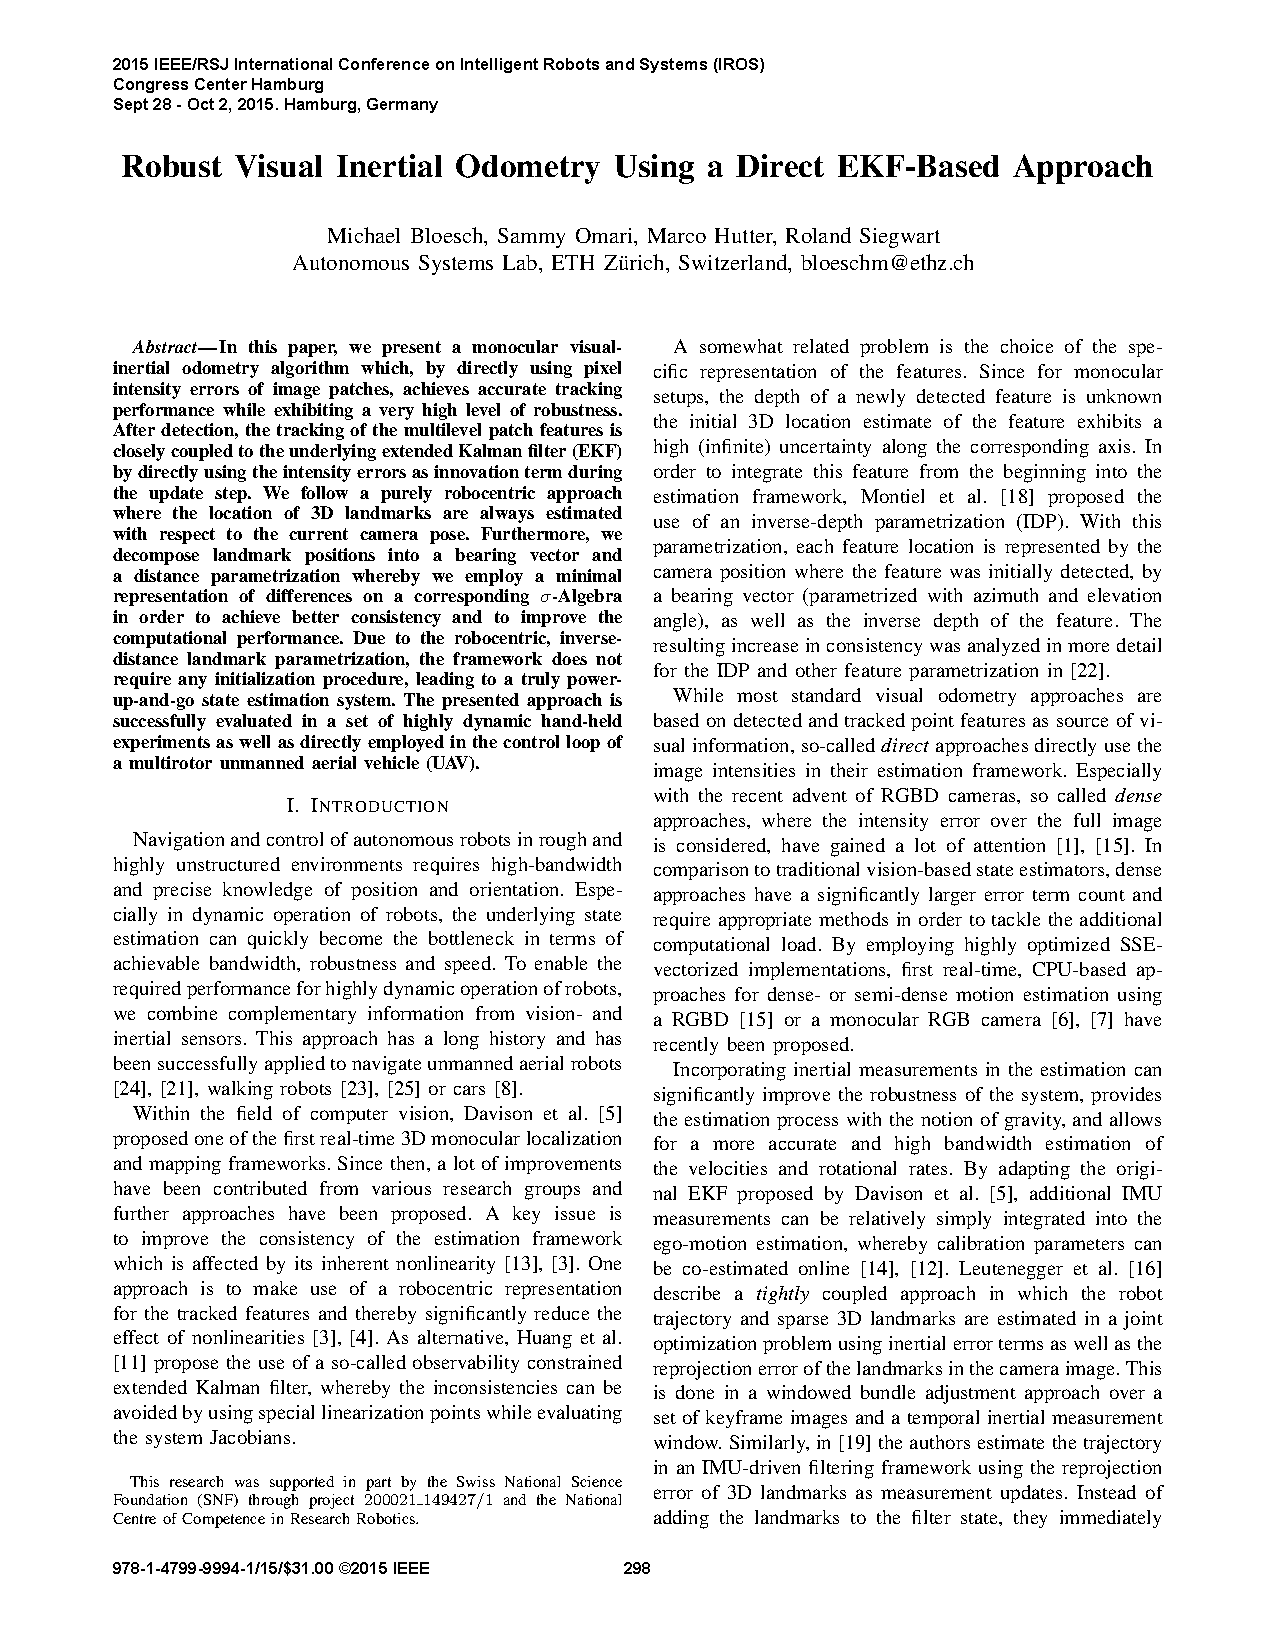
\includepdf[pages=-,scale=.8,pagecommand={}]{chap8_scene_reconstruction/papers/BloeschOmariHutter15.pdf}

%------------------------------------------------
\section{Building a Voxel Map}
\label{sec:voxel_map_updates}

\rwbcomment{Need to rewrite this section.}

\marginnote{This section is inspired by a similar discussion in (Thrun, 2006)\cite{ThrunBurgardFox06}.}
Associated with every voxel in the rolling voxel world is a probability that the voxel is occupied by an object.  The probability that a voxel is occupied at time $k$ will be a function of the output of the vision sensor at times $k, k-1, \dots, 0$.  Let $X_\ell[k]$ be a binary random variable representing the state of the $\ell^{th}$ voxel at time $k$, with the following possible values:
\[
X_\ell[k] = \begin{cases}
	\text{O} & \text{~meaning voxel $\ell$ is occupied with an object at time $k$} \\
	\text{E} & \text{~meaning voxel $\ell$ is empty at time $k$}
\end{cases}. 
\]
Let $Z_{\ell}[k]$ be a binary random variable representing the measurement of the $\ell^{th}$ voxel at time $k$ with the following possible value:
\[
Z_\ell[k] = \begin{cases}
\text{O} & \text{~meaning the sensor measures an object in voxel $\ell$ at time $k$} \\
\text{E} & \text{~meaning the sensor does not measure an object in voxel $\ell$ at time $k$}
\end{cases}.
\]

Let
\[
\pi_\ell[k] = P(X_\ell[k] = \text{O}|Z_\ell[k:0]).
\]
Using Bayes law $P(A|B,C) = \frac{P(B|A,C)P(A|C)}{P(B|C)}$ we get that
\begin{align*}
P(X_\ell[k] = \text{O}~|~Z_\ell[k:0]) &= \frac{P(Z_\ell[k] ~|~ X_\ell[k] = \text{O}, Z_\ell[k-1:0])P(X_\ell[k] = \text{O}~|~ Z_\ell[k-1:0])}{P(Z_\ell[k] ~|~ Z_\ell[k-1:0])} \\
&= \frac{P(Z_\ell[k] ~|~ X_\ell = \text{O})P(X_\ell[k] = \text{O}~|~ Z_\ell[k-1:0])}{P(Z_\ell[k] ~|~ Z_\ell[k-1:0])},
\end{align*}
where
\begin{align*}
P(Z_\ell[k] ~|~ Z_\ell[k-1:0]) 
	&= P(Z_\ell[k] ~|~ X_\ell[k] = \text{O}, Z_\ell[k-1:0])P(X_\ell[k] = \text{O}~|~ Z_\ell[k-1:0]) 
	\\ &\quad
	+ P(Z_\ell[k] ~|~ X_\ell = \text{E}, Z_\ell[k-1:0])P(X_\ell[k] = \text{E}~|~ Z_\ell[k-1:0]) \\
	&= P(Z_\ell[k] ~|~ X_\ell[k] = \text{O})P(X_\ell[k] = \text{O}~|~ Z_\ell[k-1:0]) 
	\\ &\quad
	+ P(Z_\ell[k] ~|~ X_\ell[k] = \text{E})P(X_\ell[k] = \text{E}~|~ Z_\ell[k-1:0]),
\end{align*}
and where we have used the assumption that the measurement at time $k$ only depends on the state at time $k$.
Define the {\em a priori} probability as
\[
\bar{\pi}_\ell[k] \defeq P(X_\ell[k] = \text{O}|Z_\ell[k-1:0]),
\]
and also define the probability of detection and probability of false alarm as
\begin{align*}
p_D &\defeq P(Z_\ell[k]=\text{O} ~|~ X_\ell[k]=\text{O}) \\
p_{FA} &\defeq P(Z_\ell[k]=\text{O} ~|~ X_\ell[k]=\text{E}),
\end{align*}
then the probability update law becomes
\[
\pi_\ell[k] = \begin{cases}
\frac{p_D \bar{\pi}_\ell[k]}{p_D\bar{\pi}_\ell[k]+p_{FA}(1-\bar{\pi}_\ell[k])} &\quad Z_k=\text{O} \\
\frac{(1-p_D) \bar{\pi}_\ell[k]}{(1-p_D)\bar{\pi}_\ell[k]+(1-p_{FA})(1-\bar{\pi}_\ell[k])} &\quad Z_k=\text{E}
\end{cases}.
\]
The {\em a priori} probability of occupancy is given by
\begin{align*}
\bar{\pi}_\ell[k] &= P(X_\ell[k] = \text{O}|Z_\ell[k-1:0]) \\
&= P(X_\ell[k] = \text{O}~|~ X_\ell[k-1]=\text{O}, Z_\ell[k-1:0])
   P(X_\ell[k-1] = \text{O}~|~Z_\ell[k-1:0]) 
   \\ &\quad
 + P(X_\ell[k] = \text{O}~|~ X_\ell[k-1]=\text{E}, Z_\ell[k-1:0])
   P(X_\ell[k-1] = \text{E}~|~Z_\ell[k-1:0]) \\
&= P(X_\ell[k] = \text{O}~|~ X_\ell[k-1]=\text{O})
   \pi_\ell[k-1]
   \\ &\quad
 + P(X_\ell[k] = \text{O}~|~ X_\ell[k-1]=\text{E})
   (1-\pi_\ell[k-1]),
\end{align*}
where we have used the assumption that state transitions do not depend on the measurements.  Define the static and transition probabilities as
\begin{align*}
p_{s} &= P(X_\ell[k] = \text{O}~|~ X_\ell[k-1]=\text{O}) \\
p_ {t}&= P(X_\ell[k] = \text{O}~|~ X_\ell[k-1]=\text{E}),
\end{align*}
then the {\em a priori} probability is given as
\[
\bar{\pi}_\ell[k] = p_{s}\pi_\ell[k-1] + p_{t}(1-\pi_\ell[k-1]).
\]
If voxel $\ell$ is not measured at time $k$, then 
\[
P(X_\ell[k]=O ~|~ Z_\ell[0:k]) = P(X_\ell[k]=O ~|~ Z_\ell[0:k-1]),
\]
which implies that
\[
\pi_\ell[k] = \bar{\pi}_\ell[k].
\]

In summary we have the following result.
\begin{lemma}
	Define the probability of detection $p_{_D}$, the probability of false alarm $p_{_{FA}}$, the probability of a static voxel $p_{s}$, and the probability of a transitioning voxel $p_{t}$ as
	\begin{align*}
		p_{_D} &= P(Z_\ell[k]=\text{O} ~|~ X_\ell[k]=\text{O}) \\
		p_{_{FA}} &= P(Z_\ell[k]=\text{O} ~|~ X_\ell[k]=\text{E}), \\
		p_s &= P(X_\ell[k] = \text{O}~|~ X_\ell[k-1]=\text{O}) \\
		p_t &= P(X_\ell[k] = \text{O}~|~ X_\ell[k-1]=\text{E}).
	\end{align*}
	Then the optimal Bayes filter for the $\ell^{th}$ voxel cell is given by
	\begin{align*}
		\bar{\pi}_\ell[k] &= p_{s}\pi_\ell[k-1] + p_{t}(1-\pi_\ell[k-1]) \\
		\pi_\ell[k] &= \begin{cases}
		\frac{p_{_D} \bar{\pi}_\ell[k]}{p_{_D}\bar{\pi}_\ell[k]+p_{_{FA}}(1-\bar{\pi}_\ell[k])} &\quad Z_\ell[k]=\text{O} \\
		\frac{(1-p_{_D}) \bar{\pi}_\ell[k]}{(1-p_{_D})\bar{\pi}_\ell[k]+(1-p_{_{FA}})(1-\bar{\pi}_\ell[k])} &\quad Z_\ell[k]=\text{E}  \\
		\bar{\pi}_\ell[k] &\quad \text{no measurement}
		\end{cases}.
	\end{align*}
	
	
\end{lemma}









